\documentclass{llncs}
\usepackage{times}
\usepackage[T1]{fontenc}

% Comentar para not MAC Users
%\usepackage[applemac]{inputenc}
\usepackage[export]{adjustbox}
\usepackage{a4}
%\usepackage[margin=3cm,nohead]{geometry}
\usepackage{epstopdf}
\usepackage{graphicx}
\usepackage{fancyvrb}
\usepackage{amsmath}
%\renewcommand{\baselinestretch}{1.5}

\begin{document}
\mainmatter
\title{Blockchain}

\titlerunning{Paper Title}

\author{João Azevedo \and Pedro Machado \and Paulo Araújo}

\authorrunning{Autor1 \and Autor2 \and Autor3}

\institute{
University of Minho, Department of  Informatics, 4710-057 Braga, Portugal\\
e-mail: \{a85227,a83719,a85729\}@alunos.uminho.pt
}

\date{}
\bibliographystyle{splncs}

\maketitle
\begin{abstract}
BlockChain é essencialmente um sistema de registo de dados, tanto para eventos digitais como para transações num registo público. Cada registo ou transação é verificado por consenso da maioria dos participantes no sistema e uma vez inserida, a informação nunca poderá ser apagada. A BlockChain apresenta-se como uma tecnologia imutável e com os seus dados distribuídos por todos os seus utilizadores, sendo estes fatores que a tornam uma tecnologia de confiança a nível de segurança.
Atualmente, as cripto-moedas (por exemplo, a Bitcoin, Ripple, Ethereum e Tether) são a implementação mais popular da BlockChain. Contudo, estes exemplos de implementação desta tecnologia são igualmente os mais controversos, pois viabilizam um mercado global de transações anónimas sem nenhum controlo governamental.
  
Este manuscrito descreve a tecnologia Blockchain e algumas aplicações específicas populares e atrativas. Procuramos também explorar oportunidades e vantagens desta tecnologia disruptiva não deixando de salientar igualmente as suas desvantagens. 


\end{abstract}

\section{Introduction}

%N‹o esquecer de referenciar apropriadamente...
%meanings~\cite{Nguyen99}. ...

Nos dias de hoje temos total \textbf{confiança} em entidades governamentais (...e não só), públicas ou privadas, que decidem como os nossos dados são partilhados, guardados e mantidos. \par 

\vspace{0.05cm}

Estas asseguram a \textbf{privacidade} dos dados e estabelecem a nossa \textbf{identidade} de tal modo que, colocámos nas mesmas a responsabilidade de gerir o nosso dinheiro e as \textbf{transações} que fazemos. Será que podemos confiar nestas instituições para decidir como transacionamos dados ou até mesmo dinheiro? - A resposta é: não sabemos! \par 

\vspace{0.05cm}

A verdade é que, como seres humanos, temos a necessidade de ter algo que nos traga conforto em \textbf{decisões} importantes como é o caso da movimentação de bens monetários.  \par

\vspace{0.05cm}

A tecnologia \textbf{\textit{Blockchain}} surge no sentido de ajudar a introduzir essa confiança, nomeadamente na área das transações económicas. Como? Através da confiança que depositámos na \textbf{tecnologia}. \par

\vspace{0.05cm}

A aplicação da \textit{Blockchain} trouxe muitos benefícios na indústria atual, a indústria 4.0, dos dados, que necessita, essencialmente, de \textbf{sistemas seguros}, \textbf{rápidos} e \textbf{imutavéis} no que toca à manutenção da identidade desses mesmos dados, pois só assim é que estes podem ser analisados com clareza e acertividade. 


\section{What is Blockchain?}

	A Blockchain é na sua raiz uma \underline{Base de Dados} que guarda registos também chamados de \underline{blocos}. Estes encontram-se ligados e são permanentemente mantidos e verificados usando criptografia, estabelecendo um histórico permanente de transações desses mesmos dados. \par
	
	\vspace{0.05cm}

	Em termos de topologia de rede, a Blockchain é utilizada numa arquitetura P2P\footnote{P2P: Do Inglês, Peer-to-Peer.} que se baseia num sistema descentralizado de partilha de informação, ou seja, não necessita de um servidor central para controlo de dados pois cada nó serve como host/servidor e como autenticador dos dados que circulam na rede. Na figura \ref{fig1} pode-se claramente ver a sua raiz descentralizada em que cada participante da rede mantém uma cópia do \textit{Ledger} para si. \par

    \vspace{0.05cm}

    \begin{figure}
    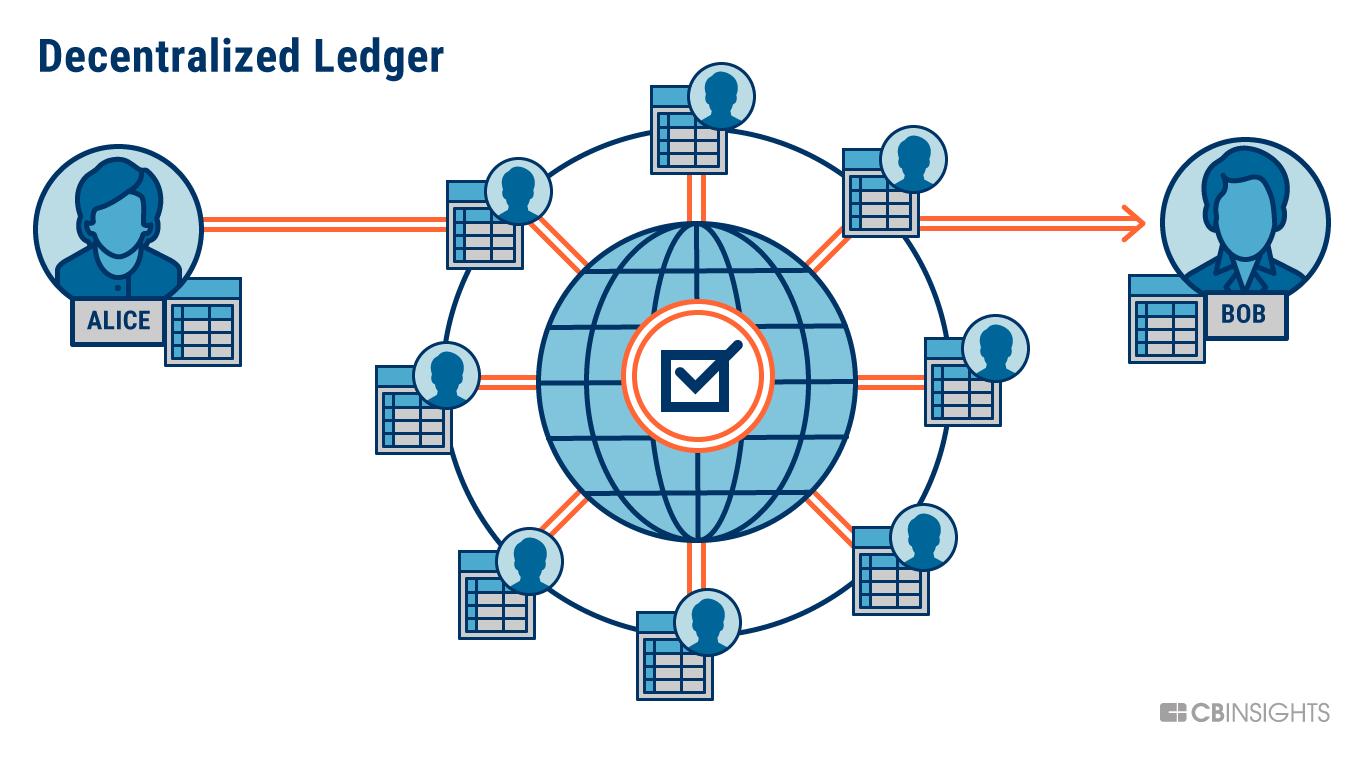
\includegraphics[width=\textwidth]{template_LNCS_Blockchain/img/modelo-descentralizado.png}
    \caption{Blockchain decentralized design. \textit{Retrieved from: cbinsights.com}} \label{fig1}
    \end{figure}
    
    \vspace{8cm}

    \vspace{0.05cm}

	Trata-se de um \textbf{sistema distribuído} que pode ser público (acessível a partir de qualquer utilizador que deseja participar na rede) ou privado (só para utilizadores com elevadas permissões de autenticação).  \par
    
    \vspace{0.05cm}

	Essencialmente, numa Blockchain pública, ou seja, num registo em cadeia de transações de dados interligados, cada elemento da rede tem uma cópia completa da Blockchain e está responsável por verificar novas transações e, em conjunto com os outros participantes, chegar a um consenso final sobre a verdade dos dados transacionados, isto é, validar as chaves criptográficas que unem os blocos da cadeia. \par

    \vspace{0.05cm}

	Partimos do princípio que, utilizando um sistema como este, os dados já registados \textbf{nunca mais poderão ser apagados ou até alterados}. Sendo assim, podemos pensar nisto como tentar roubar algo de um supermercado e estar constantemente a ser observado por pessoas, camâras de vigilância e até mesmo sensores à saída. Isto torna, deste modo, a \underline{Blockchain segura por design}. \par


\section{Blockchain Workflow - A brief process description}

	A Blockchain forma-se a partir da criação e \textit{linking}\footnote{Conexão entre blocos.} de blocos de transações partilhados por participantes da rede descentralizada.  \par

    \vspace{0.05cm}

	Os nós da rede que apenas querem registar transações de dados enviam essas transações para que estas sejam visíveis a partir de todos aqueles que as pretentem validar. Segue-se o primeiro processo de validação de uma transação. \par


\subsection{Process 1: Signing and approving the transaction}

	Aliado a cada participante da rede temos uma \textit{Private key} e uma \textit{Public key} que servem para autenticar o utilizador no sistema que usa a Blockchain para que os seus dados sejam confirmados e a transação seja devidamente assinada. \par

	\vspace{0.05cm}

    A \textit{Private key} (privada ao utilizador) é gerada aleatoriamente e a \textit{Public key} é gerada a partir da \textit{Private key}, o que a torna dificil de decifrar. \par

	No momento de adicionar uma nova transação, por exemplo de \textit{Bitcoin}\footnote{Bitcoin - Apresentada em 2008 por (ou por um grupo denominado por) Satoshi Nakamoto} neste sistema, utilizando a \textit{Public key} e os dados da transação é gerada uma assinatura que, no fundo, é como se fosse uma chave associada a essa transação.	Uma transação encontra-se processada quando uma assinatura é gerada para a mesma, por um utilizador válido. \par

\subsection{Process 2: Block crafting procedure}

	Neste momento, tendo validado transações, estas são agrupadas num Bloco, assinado com "timestamps" ou outras assinaturas digitais, e adicionadas à Blockchain. Este processo descreve a forma mais simples de validar blocos, o que não acontece no caso da Bitcoin. Nesta criptomoeda e noutras temos outros utilizadores da rede que têm a função de validar blocos criando aquilo que se chama de \textit{Proof-of-Work}.\par
	
	\vspace{0.05cm}

\textbf{\textit{Proof-of-Work - Consensus mechanism:}} O objetivo de sistemas como a Bitcoin, baseados em tecnologias como a Blockchain, é ser-se seguro e imutável, ou seja, que não permita alterações de transações já registadas. Para isso são utilizadas tecnologias de segurança criptográficas para gerar assinaturas digitais dos blocos adicionados à Blockchain. \par

    \vspace{0.05cm}

	Mediante diferentes dados, os \textit{miners}\footnote{Utilizadores que disponibilizam as suas máquinas para a validação dos blocos.} utilizam funções criptográficas para gerar uma impressão digital desse bloco que identifica unicamente o mesmo. O trabalho destes participantes da rede é, em geral, encontrar um número (chamado de "Nounce") que juntamente com os dados da transação produza uma chave criptográfica com umas dadas restrições. \par

	    \vspace{0.05cm}

No caso da Bitcoin, o trabalho dos \textit{miners} é gerar uma \textit{hash-key} que tenha um número definido de zeros no início, o que representa um trabalho computacionalmente complicado utilizando muito CPU e muita energia elétrica. Este conceito de gerar esta hash, ou seja, encontrar uma chave que valide o bloco é chamado de "Proof-of-Work".

	    \vspace{0.5cm}
	Após \textit{mining} de um bloco, ou seja, encontrarem a \textit{hash-key} correta para o mesmo, estes fazem \textit{brodcast}\footnote{Partilha.} da sua solução para toda a rede (utilizando um protocolo denominado de \textit{Gossip}) e a partir deste momento, todos os outros utilizadores param o seu trabalho para receber o novo bloco e validá-lo.

	\begin{figure}
    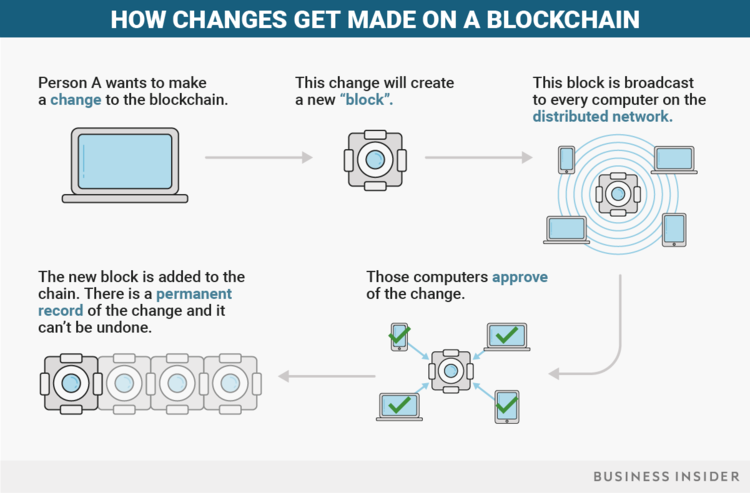
\includegraphics[scale=0.4, center]{template_LNCS_Blockchain/img/blockchain-howitworks.png}
    \caption{How changes get made on a Blockchain.} \label{fig1}
    
    \end{figure}
    \vspace{5cm}

	Validar o bloco é, essencialmente, verificar esse "Proof-of-Work", e o encadeamento lógico das transações lá registadas e assinadas. Uma vez validado o novo Bloco este é incluído na cadeia atual e ligado através de uma chave criptográfica do bloco anterior e é estabelecido que este bloco obteve uma confirmação. Estas confirmações são contadas mediante a quantidade de blocos que a partir deste foram adicionados sendo necessário 5 novos blocos a seguir a este para este receba a confirmação final, no caso da \textit{Bitcoin}.
	

%%%%%%%%%%%%%%%%%%%%%%%%%%%%%%%%%%%%%%%%%%%%%%%%%%%%%%%%%%%%%%%%%%%%%%%%%%%%%%%%%%%%5
\section{Blockchain benefits that are transforming our Society}

A criação da tecnologia Blockchain introduziu muitas aplicações em diversas indústrias com a principal vantagem de potenciar uma maior segurança em ambientes pouco confiáveis. 
	
A verdade é que esta tecnologia, apesar de ter surgido à uns bons anos, está na sua infância apenas. Felizmente, universidades, empresas, e outras corporações já estão a trabalhar na sua investigação e em experiências que têm vindo a comprovar o seu valor.

Assim sendo, seguem-se as principais vantagens introduzidas pelo sistema Blockchain:

\subsection{Advantages}
\vspace{0.05cm}
\subsubsection{Um sistema distribuído.}

	Visto que os dados armazenados relativos à Blockchain são guardados, como cópias, em milhares de dispositivos numa rede de utilizadores distribuída e descentralizada, o risco de ataques e falhas técnicas num nodo não condiciona o sistema global nem os outros nodos porque, essencialmente, não existe um ponto central mas sim um sistema distribuído de pontos.

	Em comparação, Bases de dados tradicionais contam com um conjunto reduzido de servidores que são mais vulneráveis a \textit{technical failures} e \textit{cyber attacks}.

\subsubsection{Estabilidade.}

	Blocos validados e adicionados são raramente revistos/rejeitados pois, uma vez que os dados são registados na Blockchain é extremamente difícil remover/alterar os mesmos.

	Isto torna a Blockchain uma tecnologia perfeita para guardar registos financeiros ou qualquer outros dados que requerem um histórico permanente dos mesmos porque todas as mudanças são registadas e permanetemente adicionadas numa base de dados pública e distribuída.

\subsection{Disadvantages}

Como qualquer algoritmo ou tecnologia, a BlockChain também possui características menos apreciadas. 
\paragraph{\textbf{O escalonamento de dados e o seu espaço de memória.}} Se um utilizador quiser fazer a sua primeira inserção de um bloco numa cadeia blockChain, este precisa primeiro de obter toda a cadeia de blocos já existentes e de validar o bloco antes da sua inserção. Isto poderá provocar um ‘delay’ de várias horas, pois o número de blocos tende a crescer exponencialmente. Atualmente, a blockChain da Bitcoin necessita de 200 GB de memória!
 
 \paragraph{\textbf{Computação Quântica.}}
 A blockChain baseia-se no facto de ser quase impossível um utilizador descodificar e comprometer a cadeia, devido à falta de capacidade de processamento. Contudo, com a introdução de computadores quânticos, a blockChain poderá ter a sua imutabilidade posta em causa, pois estes podem conseguir penetrar a cadeia através da “força bruta”

 \paragraph{\textbf{'51\% attack'}}. Na blockchain há uma falha de segurança conhecida como ‘51\% attack’. Caso haja mais de metade dos utilizadores com acesso à cadeia de Blockchain e sejam maliciosos, estes conseguem dominar e comprometer a cadeia Blockchain.




\subsection{Applications}

    Falar de Blockchain sem referenciar o seu benifício em criptomoedas e transações digitais é algo impensável, até porque mais de 1600 moedas digitais foram criadas até ao momento.
    Mas, para além das criptomoedas apenas temos de ter imaginação para inventar mais usos. Por exemplo, conta-kilómetros de carros? Registar automaticamente os kilómetros dos carros para prevenir que sejam adulterados esses valores e, na verdade, já está a ser desenvolvida esta aplicação pela \textbf{Bosh}\footnote{Vendedor de serviços automóvel e tecnológicos.}. \par
    
    Por outro lado podemos usar a Blockchain para guardar votos de eleições visto que toda a gente poderia ter acesso às votações, o registo temporal e criptográfico da validade dos votos e o resultado final visto que votos em papel são caros e influenciáveis.

    Registo de identidade de vendedores \textit{online} e das transações efetuadas pelos clientes seria outra grande aplicação desta tecnologia.
    
    As vantagens apresentadas falam por si e podem ser escaladas para outras aplicações futuras que nos irão, certamente, ajudar em questões relacionadas com a segurança das Bases de dados.

%%%%%%%%%%%%%%%%%%%%%%%%%%%%%%%%%%%%%%%%%%%%%%%%%%%%%%%%%%%%%%%%%%%%%%%%%%%%%%%%%%%%5
%\section{Simulation Scenario}

\section{Conclusions}

	Incertezas...é aquilo que enfrentamos hoje em dia pois não sabemos com quem estamos a trocar bens e sem ter a garantia de que vamos ter um "Plano B" caso algo corra mal.

    \vspace{0.05cm}

	Se quiser comprar algo de um sistema como o eBay, o que faço antes de comprar? Talvez ver quem é o vendedor, de onde é, a sua classificação, as "reviews", etc...Isto é o que fazemos hoje em dia para baixar as nossas incertezas sobre com quem estamos a lidar.

	    \vspace{0.05cm}

Mas mesmo assim, podemos pensar em quantos perfis podemos criar em diferentes "websites"...São perfis legítimos? Confiáveis? Somos a mesma pessoa? Estabelecemos a mesma identidade nos diferentes perfis?

    \vspace{0.05cm}

	A Blockchain não tem filtros, permite que qualquer indivíduo a utilize de onde quiser e como quiser com a garantia de que a identidade do utilizador da mesma é única e sem máscaras. Facilmente poderíamos ver a identidade de um vendedor, no caso do eBay, os seus atributos e registos todos, desde o primeiro. O que nos ajudava a decidir se valia ou não a pena comprar um dado produto do mesmo.

	    \vspace{0.05cm}

E se não receber o produto? Posso ter o meu dinheiro de volta? A Blockchain permite também a criação de contratos que são chamados caso necessário sem que uma entidade \textit{third-party} os force a tal. Só quando forem verificadas todas a condições da transação, ou seja, a validação, o contrato, é que o dinheiro pode ser realmente transacionado.

    \vspace{0.05cm}

É de realçar também que estamos a viver um mundo em que instituições autónomas e distribuídas estão empenhadas em utilizar tecnologias onde ninguém precisa de confiar em ninguém diretamente para crescer e saber a verdade dos seus dados, sendo que a incerteza (humana) nos trouxe muitas certezas (criptográficas) nesta área. 


    Por isso, estando num mundo com cada vez mais exigências de segurança, principalmente porque este tema, a segurança na Internet, é aquele que evolui menos, é importante considerar tecnologias como a Blockchain para garantir a verdade e imutabilidade da nossa identidade e dos nossos dados.

%UNCOMMENT para a bibliografia 
%% ficheirodebibliografia.bib
%\bibliography{ficheirodebibliografia}

%ou inserir directamente os v‡rios \bibitem

\begin{thebibliography}{1}
\bibitem{IBM}
What is Blockchain?, IBM.
\newblock {Inspired by ibm.com/blockchain/what-is-blockchain}

\bibitem{Nguyen99}
CROSBY, M., PATTANAYAK, P., VERMA, S. AND KALYANARAMAN, V.
BlockChain Technology: Beyond Bitcoin. Applied Inovation Review, June 2016. issue No. 2

\bibitem{TED}
Inspired by: Warburg, Bettina : Talk autor |
\newblock{"How the blockchain will radically transform the economy."}
\newblock{TEDTalks 2016 from TED conference.}

\bibitem{YOUTUBE}
3Blue1Brown.(07/07/2017).Retrieved from youtube.com/3Blue1Brown, title.: "But how does bitcoin actually work?".

\bibitem{}
Blockchain. In Wikipedia. Retrieved from https://en.wikipedia.org/wiki/Blockchain

\bibitem{}
Blockchain Gossip Protocol. Mentioned this protocol, source: www.zurich.ibm.com/dccl/papers/renesse dccl.pdf

\bibitem{}
January-February 2017 Harvard Business Review. The truth about Blockchain. Inspired by the paragraph "Guiding your aproach to Blockchain investment" in page 10.

\bibitem{}
Figure 1: Blockchain Decentralized. Source: cbinsights.com/research/what-is-blockchain-technology/

\bibitem{}
Figure 2: How Blockchain works. Source: businessinsider.com/what-is-blockchain-how-does-it-work-explainer-2017-11

\end{thebibliography}

\textbf{Further learning:}
\par
\vspace{0.2cm}
\hspace{0.5cm}* Blockchain Demo. Covers Hash functions, Blocks and Blockchain demonstrations. Retrieved from: https://anders.com/blockchain/
          
            
\end{document}